\documentclass[mathserif]{beamer}
\usetheme[secheader]{pecostalk}
\graphicspath{{figs/}}                                                                                                                              


\date{December 9, 2016}
\author[Shriya Nair]{Shriya Nair}
\institute{The University of Texas at Austin}
\title[GPU Monte-Carlo pi]{Parallelization of Monte-Carlo Estimation of pi}
%\subtitle{}

\begin{document}
\begin{frame}
\begin{center}
\end{center}
\titlepage
\begin{flushright}
\end{flushright}
\end{frame}

%===============================================================================
% NEW SLIDE
%===============================================================================
\begin{frame}
\frametitle{Overview \ldots}

\begin{itemize}
\item Problem Statement
\item Overview of GPU
\item GPU Implementation and Optimizations
\item Overview of Features
\item Previous Implementations
\item Results   
\begin{itemize}
\item GPU vs CPU
\item Thrust Library vs My implementation
\end{itemize}
\item github Structure and Build System
\item What would I have done differently?
\item Conclusion
\end{itemize}

\end{frame}

%===============================================================================
% NEW SLIDE
%===============================================================================
\begin{frame}
\frametitle{Problem Statement}

The problem statement is to answer the following questions: 
\begin{itemize}
\item How fast is GPU Implementation compared to Serial implementation?
\item What optimizations can be used to make GPU Implementation faster? 
\end{itemize}
But why Monte Carlo Simulation?
\begin{itemize}
\item Popular benchmark used in Computer Architecture field  
\item Does not need any special architectural features such as lookup tables etc. 
\item Need a measure of the throughput of computation 
\end{itemize}
\end{frame}

%===============================================================================
% NEW SLIDE
%===============================================================================
\begin{frame}                                                                                                                                                                          
\frametitle{Overview of GPU}
GPUs are compute intensive devices
\begin{itemize}
\item Each GPU has many Streaming Multiprocessors (SMs) which are lightweight cores  
\item Each SM runs one block of threads. If the num of blocks > number of SMs, then, the blocks are re run on SMs
\item The maximum number of threads per block depends on the architecture.  
\end{itemize}
What does this mean to the programmer? 
The programmer is responsible for the synchronization!
The programmer generates GPU kernels. 
\begin{itemize}
\item There is a fixed maximum number of threads per block. If this is exceeded the kernel won't run. 
\item The number of threads per block is also limited.  
\end{itemize}
\end{frame}              

%===============================================================================
% NEW SLIDE
%===============================================================================
\begin{frame}                                                                                                                                                                          
\frametitle{CUDA GPU Kernels}
How can a programmer handle all the exposed parallelism?
\begin{itemize}
\item A kernel is a function that is run by each thread in an SM.  
\item The scheduler in a GPU only schedules multiple blocks and launches threads in each block but is not responsible for thread synchronization 
\item The programmer is responsible for thread synchronization and safe thread execution.  
\end{itemize}
Does it end here? NO!
\begin{itemize}
\item The programmer cannot assume the order of the execution of blocks or threads 
\item The programmer is also responsible to maintain safe execution across blocks! 
\end{itemize} 
\end{frame}              

%===============================================================================
% NEW SLIDE
%===============================================================================
\begin{frame}                                                                                                                                                                          
\frametitle{GPU contd}
Is is worth it?
\begin{itemize}
\item Yes! If the architecture is exposed a programmer has more flexibility 
\item Can explore various options such as varying number of threads, blocks, scheduling strategy 
\item Speedups reported are in the order of 10x-100x 
\end{itemize}
Example of how a kernel is launched:
%\begin{verbatim}
%kernel_name<<<num_blocks,num_threads_per_block,total_shared_memory_per_block>>>(parameters passed to kernel);
%\end{verbatim}
Note: 
\begin{itemize}
\item The parameters passed must be on GPU memory or registers. GPU cannot read CPU memory!  
\item The parameters passed are accessed by all threads in all blocks
\end{itemize} 
\end{frame}             
 
%===============================================================================
% NEW SLIDE
%===============================================================================
\begin{frame}                                                                                                                                                                          
\frametitle{Experiment Setup}
\begin{block}{Stampede Hardware}
\begin{itemize}
\item CPU: Intel Xeon E-5 
\item GPU: NVIDIA K20 
\end{itemize}
\end{block}
\begin{block}{Software}
\begin{itemize}
\item Languages used: C++ (CPU) , CUDA(GPU) 
\item Version Control: github
\item Build System: make 
\item Plots: gnuplot  
\item Other scripts to automate and extract: bash, python  
\end{itemize}
\end{block}
\end{frame}              

%===============================================================================
% NEW SLIDE
%===============================================================================
\begin{frame}                                                                                                                                                                          
\frametitle{Implementation Details}
The algorithm was divided into the following steps:
\begin{itemize}
\item Step 1: Generate a pair of random number from 0-1
\begin{itemize}
\item CPU rand function used to generate 2*samples number of random numbers  
\item Values stored in an array and passed to both CPU and GPU estimation functions
\item In GPU impl, the array is copied from CPU to GPU memory and passed to kernel
\item In the kernel, each thread with its unique thread index and block index accesses unique elements in the array
\end{itemize}
\end{itemize}
\end{frame}              

\begin{frame}                                                                                                                                                                          
\frametitle{Implementation Details contd}
\begin{itemize}
\item Step 2: Find the number of points within the quarter circle
\begin{itemize}
\item A simple compute is used in both CPU and GPU impl to check whether a point lies within the quarter circle 
\item CPU: A count is maintained and incremented when the condition is true
\item GPU: If true, the thread writes 1 to its unique location in another shared array per block
\item    :  final count is calculated by adding all the 1s 
\end{itemize}
\item Step 3: Divide by total points to get the value of pi/4
\begin{itemize}
\item CPU: Straightforward division of total values satisfying the condition by total samples 
\item GPU: The final count obtained is per block. These per block sums have to be added to get final total count 
\item    : Division by total samples is done outside the kernel by CPU because its a low cost computation
\end{itemize}
\end{itemize}
\end{frame}              
 
%===============================================================================
% NEW SLIDE
%===============================================================================
\begin{frame}                                                                                                                                                                          
\frametitle{Optimizations}
Naive implementation is slower. The programmer is responsible for juicing out the performance benefits from GPU. Here's how i did it:
\begin{itemize}
\item Calling rand function from CPU: 
\begin{itemize}
\item rand function API exists in CUDA but it is very slow and has high overhead
\item This is not fair to compare because the aim is to compare compute power and timing
\item Hence, CPU rand is used for both implementations 
\end{itemize}
Ping pong copy: 
\begin{itemize}
\item Input to perfix sum is the output of previous iteration.  
\item This means each time the output global array has to be copied to input. Global memory -global memory copy is expensive in GPU 
\item Instead, alternate input and output arrays as output and input every odd and even iteration 
\end{itemize}
\end{itemize}
\end{frame}              


\begin{frame}                                                                                                                                                                          
\frametitle{Optimizations contd}
\begin{itemize}
\item Why was 1 written to another memory instead of performing atomic adds? 
\begin{itemize}
\item Atomic adds are expensive and serialize the code 
\item GPU being a highly parallel device handles massive serialization very badly increasing latencies 
\item A technique called Parallel Prefix Sum was used to calculate sum
\end{itemize}
\item Optimizations in parallel prefix sum:  
\begin{itemize}
\item Loop unrolling: Standard optimization 
\item Warp synchronization: Once less than 32 threads were forced to run, the warp scheduler scheduled and synchronized the threads 
\item This means expensive synchronize thread calls could be avoided
\end{itemize}
\end{itemize}
\end{frame}              

%===============================================================================
% NEW SLIDE
%===============================================================================
\begin{frame}                                                                                                                                                                          
\frametitle{Previous Implementations}
The following previous work (and open source) was found:
\begin{itemize}
\item CUDA Thurst Library has fast implementations of most popular simulations and algorithms 
\item cuRand Library also provided Monte Carlo pi estimation but the authors are still fixing compilation issues in their example code. 
\item Will be comparing my implementation with that of CUDA Thrust 
\end{itemize}
\end{frame}             

\begin{frame}                                                                                                                                                                          
\frametitle{Ensuring Fairness}
\begin{block}{Note on comparison with Thrust}
\begin{itemize}
\item In Thurst implementation the very slow CUDA rand function has been used 
\item This makes it unfair to compare my implementation with Thurst 
\item Hence, another version was made which calls CUDA rand function.  
\item Still missing something: The time to allocate and free memory was also included. Now the comparison is fair.  
\end{itemize}
\end{block}
\end{frame}             
 

%===============================================================================
% NEW SLIDE
%===============================================================================
\begin{frame}                                                                                                                                                                          
\frametitle{Results: 1/3}
\begin{block}{Comparison with naive CPU Implementation}
\begin{itemize}
\item For the first few elements, CPU implementation is faster because the overhead of launching threads beats the benefits obtained from parallelism 
\item But for large number of samples, GPU implementation is approx 100x faster as shown below.
\end{itemize}
\end{block}
\end{frame}             
 
%===============================================================================
% NEW SLIDE
%===============================================================================
\begin{frame}                                                                                                                                                                          
\frametitle{Results: 2/3}

\begin{block}{Comparison with CUDA Thrust Implementation}
\begin{itemize}
\item My implementation is always faster than that of Thrust as shown below. 
\item From a glance at their code, potential for improvements were identified.  
\end{itemize}
\end{block}
\end{frame}             
 
%===============================================================================
% NEW SLIDE
%===============================================================================
\begin{frame}                                                                                                                                                                          
\frametitle{Results: 3/3}
\begin{block}{Other Observations}
\begin{itemize}
\item Number of samples per thread for the fastest time is 1 or 2.  
\item I expected an increase in performance for 4, as a tradeoff between overhead of starting threads vs serializing the code by half.  
\item But, was midly surprised to find performance degradation 
\end{itemize}
\end{block}
\end{frame}             

%===============================================================================
% NEW SLIDE
%===============================================================================
\begin{frame}                                                                                                                                                                          
\frametitle{Directory Structure and Build System}
\begin{center}
\begin{itemize}
\item Free to use
\item The following image describes the source file dependency 
\end{itemize}
\end{center}
\end{frame}             

%===============================================================================
% NEW SLIDE
%===============================================================================
\begin{frame}                                                                                                                                                                          
\frametitle{What would I have done differently?}
\begin{center}
\begin{itemize}
\item Satisfied with the general direction of the project from start
\item Always scope for improvement
\item Could have explored non open source fast implementations 
\item Could have modified thrust library, but implementing from scratch was much more fun!
\item Could have given more flexibility to user 
\begin{itemize}
\item number of blocks, number of threads to be user defined         
\item But will have to sacrifice warp scheduling  
\end{itemize}
\end{itemize}
\end{center}
\end{frame}             

%===============================================================================
% NEW SLIDE
%===============================================================================
\begin{frame}                                                                                                                                                                          
\frametitle{Conclusion}
\begin{center}
\begin{itemize}
\item Could exploit massive parallelism in GPU to beat Thrust implementation 
\item Good learning experience, confident as a multicore programmer!
\item Could not have done without github
\item Every researcher has a tendency to look for favourable results overlooking unfairness: Taught me a lesson to do fair comparisons 
\end{itemize}
\end{center}
\end{frame}             

%===============================================================================
% NEW SLIDE
%===============================================================================
\begin{frame}
\frametitle{Example 1: 2 Blocks with nested item lists}
%===============================
\begin{block}{First Block}
\begin{itemize}
\item First Item
	\begin{itemize}
	\item Subitem
	\end{itemize}
\item Second Item:
	\begin{itemize}
	\item More subitems
	\item And more
	\end{itemize}
\end{itemize}
\end{block}
%===============================
\begin{block}{Second Block}
\begin{itemize}
\item With an item
\end{itemize}
\end{block}
%===============================
\end{frame}






%===============================================================================
% NEW SLIDE
%===============================================================================
\begin{frame}
\frametitle{Example 2: 2 Columns;\\ one column with two blocks, one block with two columns!}
\begin{columns}[c]
\begin{column}{5cm}
\begin{block}{Block 1}
\begin{columns}[t]
\begin{column}{2.25cm}
\begin{itemize}
\item item 1\\
\item item 2\\
\item item 3\\
\end{itemize}
\end{column}
\begin{column}{2.75cm}
\begin{itemize}
\item item 4\\
\item item 5\\
\item item 6\\
\end{itemize}
\end{column}
\end{columns}
\end{block}
\begin{block}{Block 2}
\begin{itemize}
\item item A\\
\item item B\\
\end{itemize}
\end{block}
\end{column}
\begin{column}{5cm}
\begin{block}{Block 3}
\begin{itemize}
\item item a\\
\item item b\\
\item item c\\
\item item d\\
\end{itemize}
\end{block}
\end{column}
\end{columns}
\end{frame}
%===============================================================================
% NEW SLIDE
%===============================================================================
\begin{frame}                                                                                                                                                                          
\frametitle{Image and Bullet points}
\begin{center}
\includegraphics[width=.8\linewidth]{generic_pyramid}\\
\begin{itemize}
\item Validation is done repeatedly with increasingly complex scenarios
\item Validation pyramid may be recursive
\end{itemize}
\end{center}
\end{frame}              
%===============================================================================
% NEW SLIDE
%===============================================================================
\begin{frame}
\frametitle{Two Blocks with added text for emphasis}

{\color{pecos2}V\&V-UQ framework \emph{requires} experimental data}
\begin{block}{Calibration of component model parameters}
\begin{itemize}
\item Thermochemistry (e.g. kinetic parameters)
\item Radiation (e.g. absorptions \& emissions)
\item Turbulence (e.g. model constants)
\item Ablation (e.g. kinetic parameters)
\end{itemize}
\end{block}
\begin{block}{Validation}
\begin{itemize}
\item Component and subcomponent models
\item Coupling between models
\item Full system
\end{itemize}
\end{block}
\end{frame}

%===============================================================================
% NEW SLIDE
%===============================================================================
\begin{frame}                                                                                                                                                                          
\frametitle{1 Block and 1 Image in Column format}
\begin{columns}[c]
\begin{column}{5cm}
\begin{block}{Extensive experimental data}
\begin{itemize}
\item {\color{pecos6}Space Act Agreement}
\begin{itemize}
\item Ames EAST
\item Langley RCS
\item Ames \& JSC Arc Jets
\item AEDC T9
\item CUBRC
\item Cal Tech
\end{itemize}
\item Legacy data
\item Sandia
\item PECOS
\end{itemize}
\end{block}
\end{column}
\begin{column}{5cm}
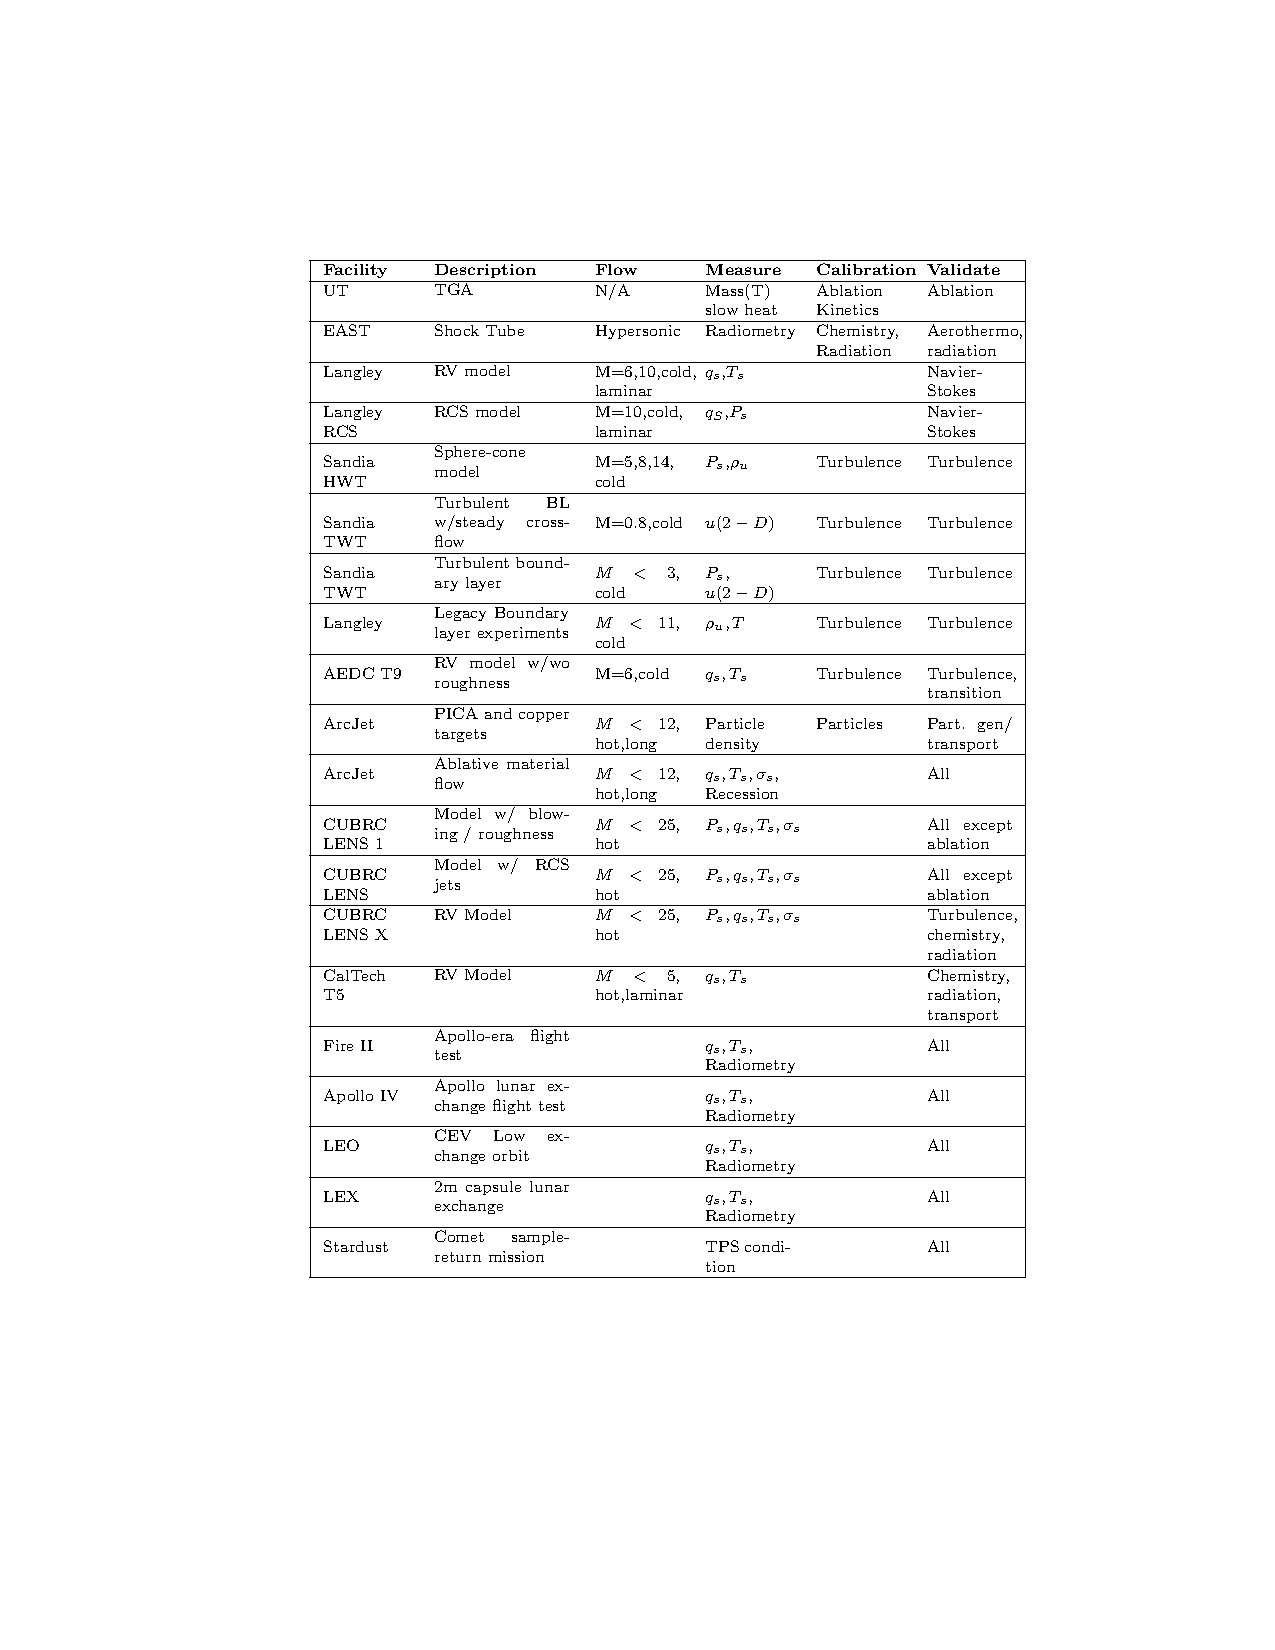
\includegraphics[scale=0.45]{validation_table}
\end{column}
\end{columns}
\end{frame}

%===============================================================================
% NEW SLIDE
%===============================================================================
\begin{frame}                                                                                                                                                                          
\frametitle{1 image and 1 itemized Block}
\begin{center}
\includegraphics[width=.5\linewidth]{pyramid_east}\\
\end{center}
\begin{block}{Goals}
\begin{itemize}
\item Calibrate and (in)validate a two-temperature thermochemical model  
\item Investigate implementation of the validation cycle with QUESO  %
\item Develop a 1D problem for future exploration of adjoints
\end{itemize}
\end{block}
\end{frame}

%===============================================================================
% NEW SLIDE
%===============================================================================
\begin{frame}                                                                                                                                                                          
\frametitle{Block and then Two Images in a Column}
\vspace {-1 mm}
\begin{block}{Facility}
\begin{itemize}
\item LENS I HST
  \begin{itemize}
  \item Variable Re reflected shock tunnel
  \item Tests: Perfect gas data, enthalpy effects, distributed roughness, roughness w/ blowing,  high-fidelity
  \end{itemize}
\item LENS XX
  \begin{itemize}
  \item Variable Re shock expansion tunnel
  \item Tests: Facility and measurement capabilities similar to EAST
  \end{itemize}
\item Visit planned for May 2009
\end{itemize}
\end{block}

\begin{columns}
  \begin{column}[l]{0.45\linewidth}
  \begin{figure}[h]
  \begin{center}
  \vspace {-5 mm}
  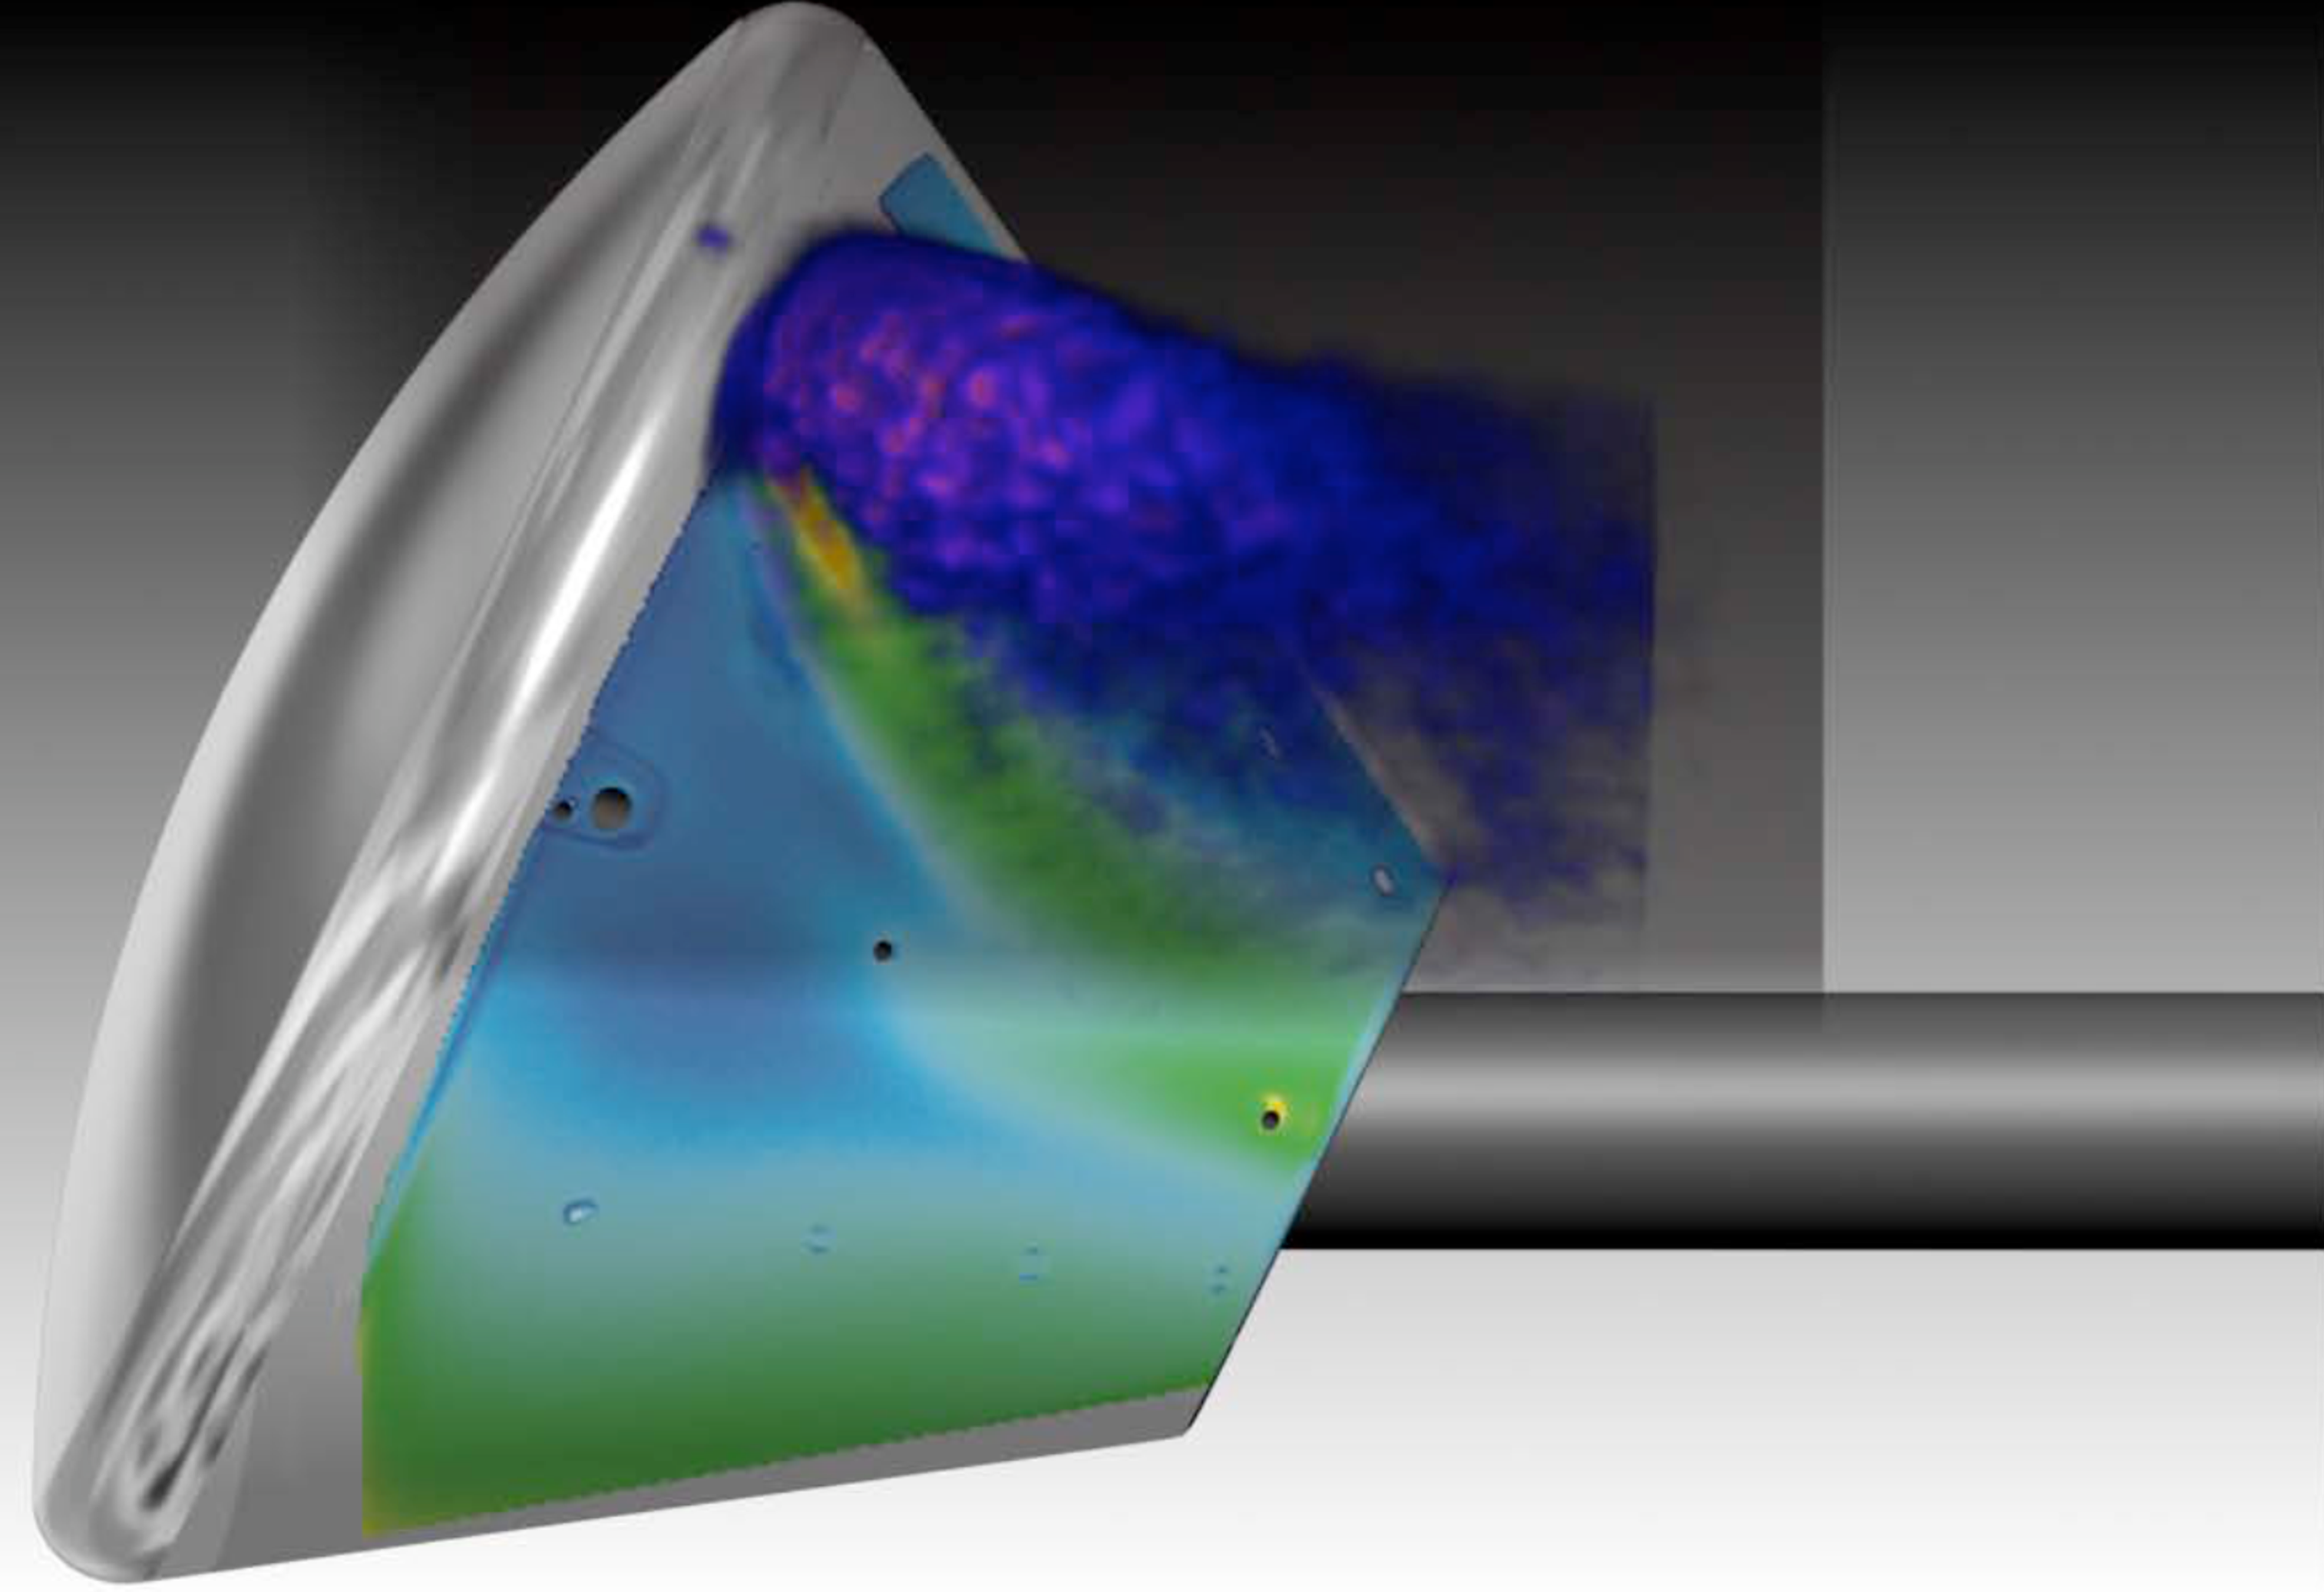
\includegraphics[width=0.9\linewidth]{RCS_PLIF.pdf} %This figure shows an RCS jet experiment at LaRC; low enthalpy vs. high enthalpy at CUBRC
  \end{center}
  \end{figure}
  \end{column}

  \begin{column}[r]{0.45\linewidth}
  \begin{figure}[h]
  \begin{center}
  \vspace {-5 mm}
  \includegraphics[width=0.9\linewidth]{LENSXX_components.pdf} %This figure shows some components of the new LENS XX facility
  \end{center}
  \end{figure}
  \end{column}
\end{columns}
\end{frame}

%===============================================================================
% NEW SLIDE
%===============================================================================
\begin{frame}
\frametitle{Two Images in Two Blocks in a Column}
\begin{columns}[c]
\begin{column}{5.5cm}
\begin{block}{Surface Ablation Rate}
\includegraphics[width=5.5cm]{surface_ablation_rate_node_valued_coarse_mesh.png}
\end{block}
\end{column}
\begin{column}{5.5cm}
\begin{block}{Surface Heat Flux}
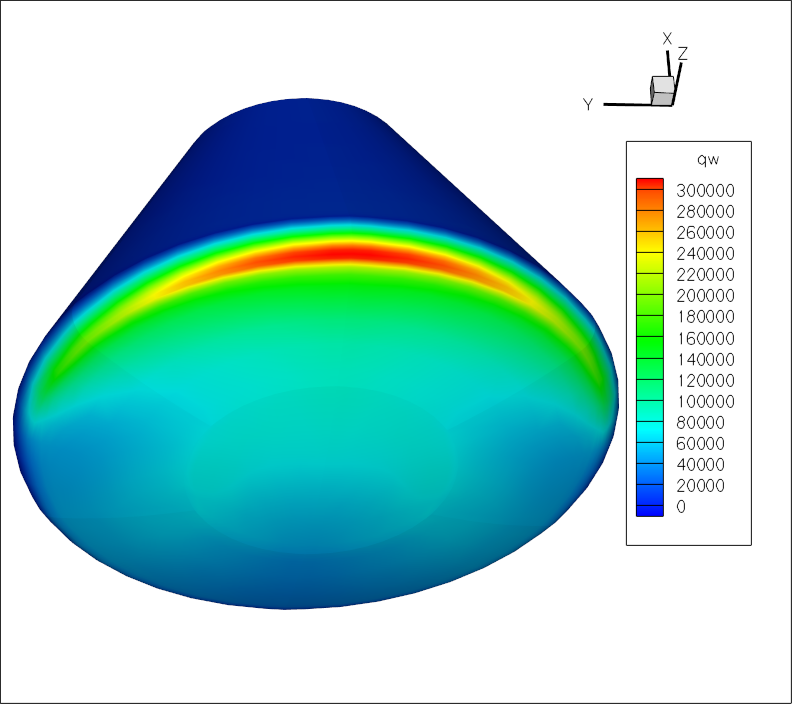
\includegraphics[width=5.5cm]{surface_heat_flux_coarse_mesh.png}
\end{block}
\end{column}
\end{columns}
\end{frame}


%===============================================================================
% NEW SLIDE
%===============================================================================
\begin{frame}                                                                                                                                                                          
\frametitle{Fancy Block / Column work}
\begin{block}{Goals}
\begin{itemize}
\item Demonstrate capability to couple ablation and radiation models with
existing hypersonic code (DPLR)
\item Evaluate sensitivity of the ablation rate and peak heat flux (QoIs)
\begin{itemize}
\item Identify most important models
\item Evaluate utility of surrogate quantities of interest
\end{itemize}
\end{itemize}
\end{block}
\begin{block}{Coupled hypersonic flow for LEO and lunar reentry, including:}
\begin{footnotesize}
\begin{columns}[T]
\begin{column}{5cm}
\begin{itemize}
\item Arrhenius chemistry
\item Gray temperature dependent radiation
\item Algebraic(Baldwin-Lomax) turbulence models
\end{itemize}
\end{column}
\begin{column}{5cm}
\begin{itemize}
\item Thermal nonequilibrium
\item Single phase flow (i.e. no particles)
\end{itemize}
\end{column}
\end{columns}
\begin{itemize}
\item 1-dimensional solid-phase ablation with ad hoc kinetics (as in CMA, FIAT, Chaleur)
\item Equilibrium surface chemistry
\end{itemize}
\end{footnotesize}
\end{block}
\end{frame}


%===============================================================================
% NEW SLIDE
%===============================================================================
\begin{frame}
\frametitle{}
\begin{block}{}
\center{Thank you!} \\
\center{Questions?}
\end{block}
\end{frame}

 
\end{document}
